%%%%%%%%%%%%%%%%%%%%%%%%%%%%%%%%%%%
%% Uso de la clase ITTol-Tesis
%%%%%%%%%%%%%%%%%%%%%%%%%%%%%%%%%%%
\documentclass[12pt]{ITTol-Tesis}


% Paquete usado para incluir texto falso (Lorem Ipsum) en el ejemplo 
\usepackage{lipsum}					

% Para links sin decoración
%\hypersetup{colorlinks=false,allbordercolors=white}

\titulo{Título de la Tesis}
\autor{Autor de la Tesis}
\grado{Maestro en Ciencias en Ciencias de la Ingeniería}
\date{Octubre de 2018}
\director{Director de la Tesis}
\codirector{Codirector de la Tesis}                                         % Si existe un codirector
%\tutor{Tutor}                                                                         % Si existe un tutor
\autorizacion{autorizacion-Tesis}                                           % Archivo de Autorización de Tesis (imagen png, pdf,jpg) 
\DeclareGraphicsExtensions{.pdf,.png,.jpg}
%\graphicspath{{./figuras/}}


%%%%%%%%%%%%%%%%%%%%%%%%%%%%%%%%%%%
%% Documento
%%%%%%%%%%%%%%%%%%%%%%%%%%%%%%%%%%%
\begin{document}

\maketitle	                                                                            % Crea la carátula
\frontmatter

\insertarautorizacion                                                            % Autorización

\begin{dedicatoria}                                                              % Dedicatoria
\begin{center}
Escriba aquí su dedicatoria.
\end{center}
\end{dedicatoria}

\begin{abstract}                                                                   % Resumen en español
\lipsum[1-2]
\end{abstract}

\selectlanguage{english}                                                     % Resumen en inglés
\begin{abstract}
\lipsum[1-2]
\end{abstract}

\selectlanguage{spanish}
\begin{agradecimientos}                                                     % Agradecimientos
\begin{center}
\textbf{AGRADECIMIENTOS}
\end{center}
\lipsum[1-3]
\end{agradecimientos}

\tableofcontents                                                                   % Índice de Contenido
{\noskip\listoffigures}                                                            % Índice de Figuras
{\noskip\listoftables}                                                             % Índice de Tablas

\mainmatter

%% Capítulos
%%%%%%%%%%%%%%%%%%%%%%%%%%%%%%%%%%%
%%%%%%%%%%%%%%%%%%%%%%%%%%%%%%%%%%%%%%%%%%%%%%%%%%%%%%%%%%%%
%% Capítulo 1 / Introducción
%%%%%%%%%%%%%%%%%%%%%%%%%%%%%%%%%%%%%%%%%%%%%%%%%%%%%%%%%%%%
\chapter{Introducción}
\epigrafe{Everyone in this country should learn how to program a computer, because it teaches you how to think.}
              {\textsc{Steve Jobs}}

\textcolor{gray}{Es el contenido global de lo que va a encontrarse en el trabajo. Incluye los aspectos relevantes de los antecedentes, la definición del problema, la justificación, los objetivos: general y específicos. En este apartado se iniciará la paginación principal con números arábigos (los capítulos podrán ir numerados con arábigos)}

%%%%%%%%%%%%%%%%%%%%%%%%%%%%%%%%%%%%%%%%%%%%%%%%%%%%%%%%%%%%
\section{Ejemplo Figura}
\lipsum[1] 
Como se puede apreciar en la Figura \ref{fig:01_Proceso}.

\begin{figure}[htbp]                                                      % Inclusión de una figura
\centering
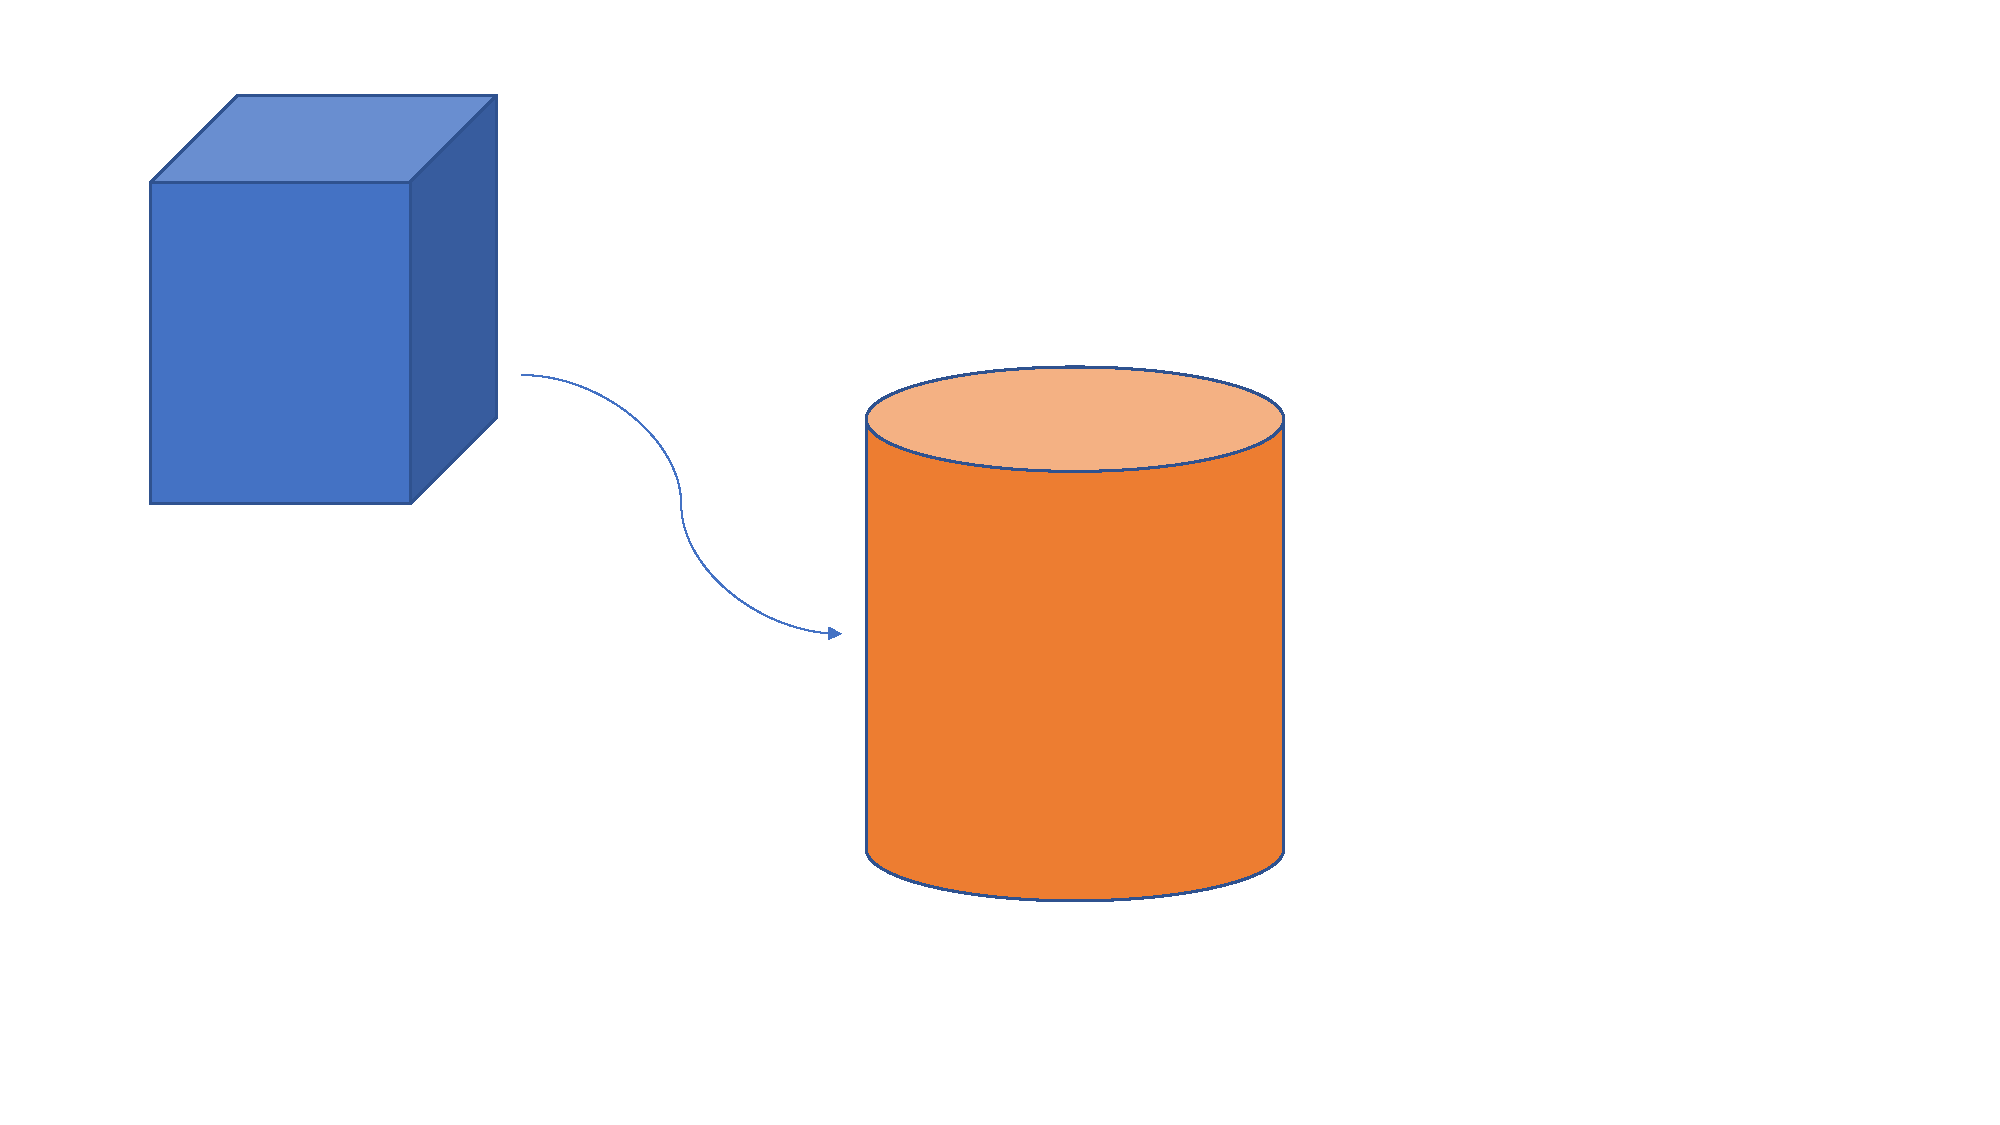
\includegraphics[width=0.80\textwidth]{a_Imagen01}
\caption{Donec vehicula augue eu neque.}
\label{fig:01_Proceso}
\end{figure}

\lipsum[2]


%%%%%%%%%%%%%%%%%%%%%%%%%%%%%%%%%%%%%%%%%%%%%%%%%%%%%%%%%%%%
\section{Ejemplo Link}
\lipsum[3-4]
En el \href{https://es.wikipedia.org/wiki/Proceso_(ingenier%C3%ADa)}{Wikipedia - Proceso} se pueden consultar la descripción
del proceso mostrado en la Figura~\ref{fig:01_Proceso}. 
                                                       % Introducción.tex
%%%%%%%%%%%%%%%%%%%%%%%%%%%%%%%%%%%%%%%%%%%%%%%%%%%%%%%%%%%%
%% Capítulo 2 / Fundamentos Teóricos y Problemática
%%%%%%%%%%%%%%%%%%%%%%%%%%%%%%%%%%%%%%%%%%%%%%%%%%%%%%%%%%%%
\chapter{Fundamentos Teóricos y Problemática}
\epigrafe{Everyone in this country should learn how to program a computer, because it teaches you how to think.}
              {\textsc{Steve Jobs}}

\section{Ejemplo Ecuación}

\lipsum[1]

\begin{equation}                                                     
\mathrm{e}^{x} = \sum_{k=0}^{\infty} \frac{x^k}{k!} = 
1 + x + \frac{x^2}{2} + \frac{x^3}{6} + \cdots
\label{eq:taylor}
\end{equation}

La ecuación \eqref{eq:taylor} muestra la expansión en serie de Taylor alrededor de $x = 0$ para la función exponencial natural.

\section{Ejemplo Cita Bibliográfica}
\lipsum[3-4].  
Los fundamentos también pueden revisarse en \cite{knuth97}. 

\section{Tercera sección}
\lipsum[5-6]
                                % Fundamento.tex
%%%%%%%%%%%%%%%%%%%%%%%%%%%%%%%%%%%%%%%%%%%%%%%%%%%%%%%%%%%%
%% Capítulo 3 / Estado del Arte
%%%%%%%%%%%%%%%%%%%%%%%%%%%%%%%%%%%%%%%%%%%%%%%%%%%%%%%%%%%%
\chapter{Estado del Arte}
\epigrafe{Everyone in this country should learn how to program a computer, because it teaches you how to think.}
              {\textsc{Steve Jobs}}

\section{Primera sección }
\lipsum[1]

\section{Ejemplos Citas Bibliográficas}
\lipsum[3-4].
Actualmente existen las siguiente propuestas de \cite{lopez2013impacto} y \cite{orduna2016revolucion}.

\section{Tercera sección}
\lipsum[5-6]
                                                         % Estado del Arte
%%%%%%%%%%%%%%%%%%%%%%%%%%%%%%%%%%%%%%%%%%%%%%%%%%%%%%%%%%%%
%% Capítulo 4 / Metodología
%%%%%%%%%%%%%%%%%%%%%%%%%%%%%%%%%%%%%%%%%%%%%%%%%%%%%%%%%%%%
\chapter{Metodología}
\epigrafe{Everyone in this country should learn how to program a computer, because it teaches you how to think.}
              {\textsc{Steve Jobs}}

\section{Primera sección}
\lipsum[1-2]. 
Se recomienda atender las recomendaciones y buena prácticas indicadas en su seminario de investigación, de tesis, o de
las referencias bibliográficas pertinentes, por ejemplo \cite{Sampieri}. 

\section{Ejemplo Algoritmo}
\lipsum[3]
\lipsum[4].
El análisis de datos se realiza con el Algoritmo \ref{Alg:Algo-01}, descrito en seguida:

\begin{algorithm}[H]
  \SetAlgoLined
  \KwData{this text}
  \KwResult{how to write algorithm with \LaTeX2e }
  initialization\;
  \While{not at end of this document}{
    read current\;
    \eIf{understand}{
      go to next section\;
      current section becomes this one\;
      }{
      go back to the beginning of current section\;
      }
    }
  \caption{How to write algorithms}
  \label{Alg:Algo-01}
\end{algorithm}

\section{Tercera sección}
\lipsum[5-6]

                                                       % Metodología
%%%%%%%%%%%%%%%%%%%%%%%%%%%%%%%%%%%%%%%%%%%%%%%%%%%%%%%%%%%%
%% Capítulo 5 / Resultados
%%%%%%%%%%%%%%%%%%%%%%%%%%%%%%%%%%%%%%%%%%%%%%%%%%%%%%%%%%%%
\chapter{Resultados}
\epigrafe{Everyone in this country should learn how to program a computer, because it teaches you how to think.}
              {\textsc{Steve Jobs}}

\section{Ejemplo Tabla}
\lipsum[1].  
Los resultados pueden verse en la Tabla \ref{tab:Tabla1}

\begin{table}[htbp]
\centering
\caption{Resultados obtenidos.}
\label{tab:pversust}
\begin{tabular}{ccc}
\toprule
\textbf{Parametro A } & \textbf{Resultado } \\
\midrule
A & 1 \\
B & 2 \\ 
C & 3 \\
D & 4 \\
\bottomrule
\end{tabular}
\label{tab:Tabla1}
\end{table}

\lipsum[2]

\section{Ejemplo Figura}
\lipsum[3-4]

\begin{figure}[htbp]
\centering
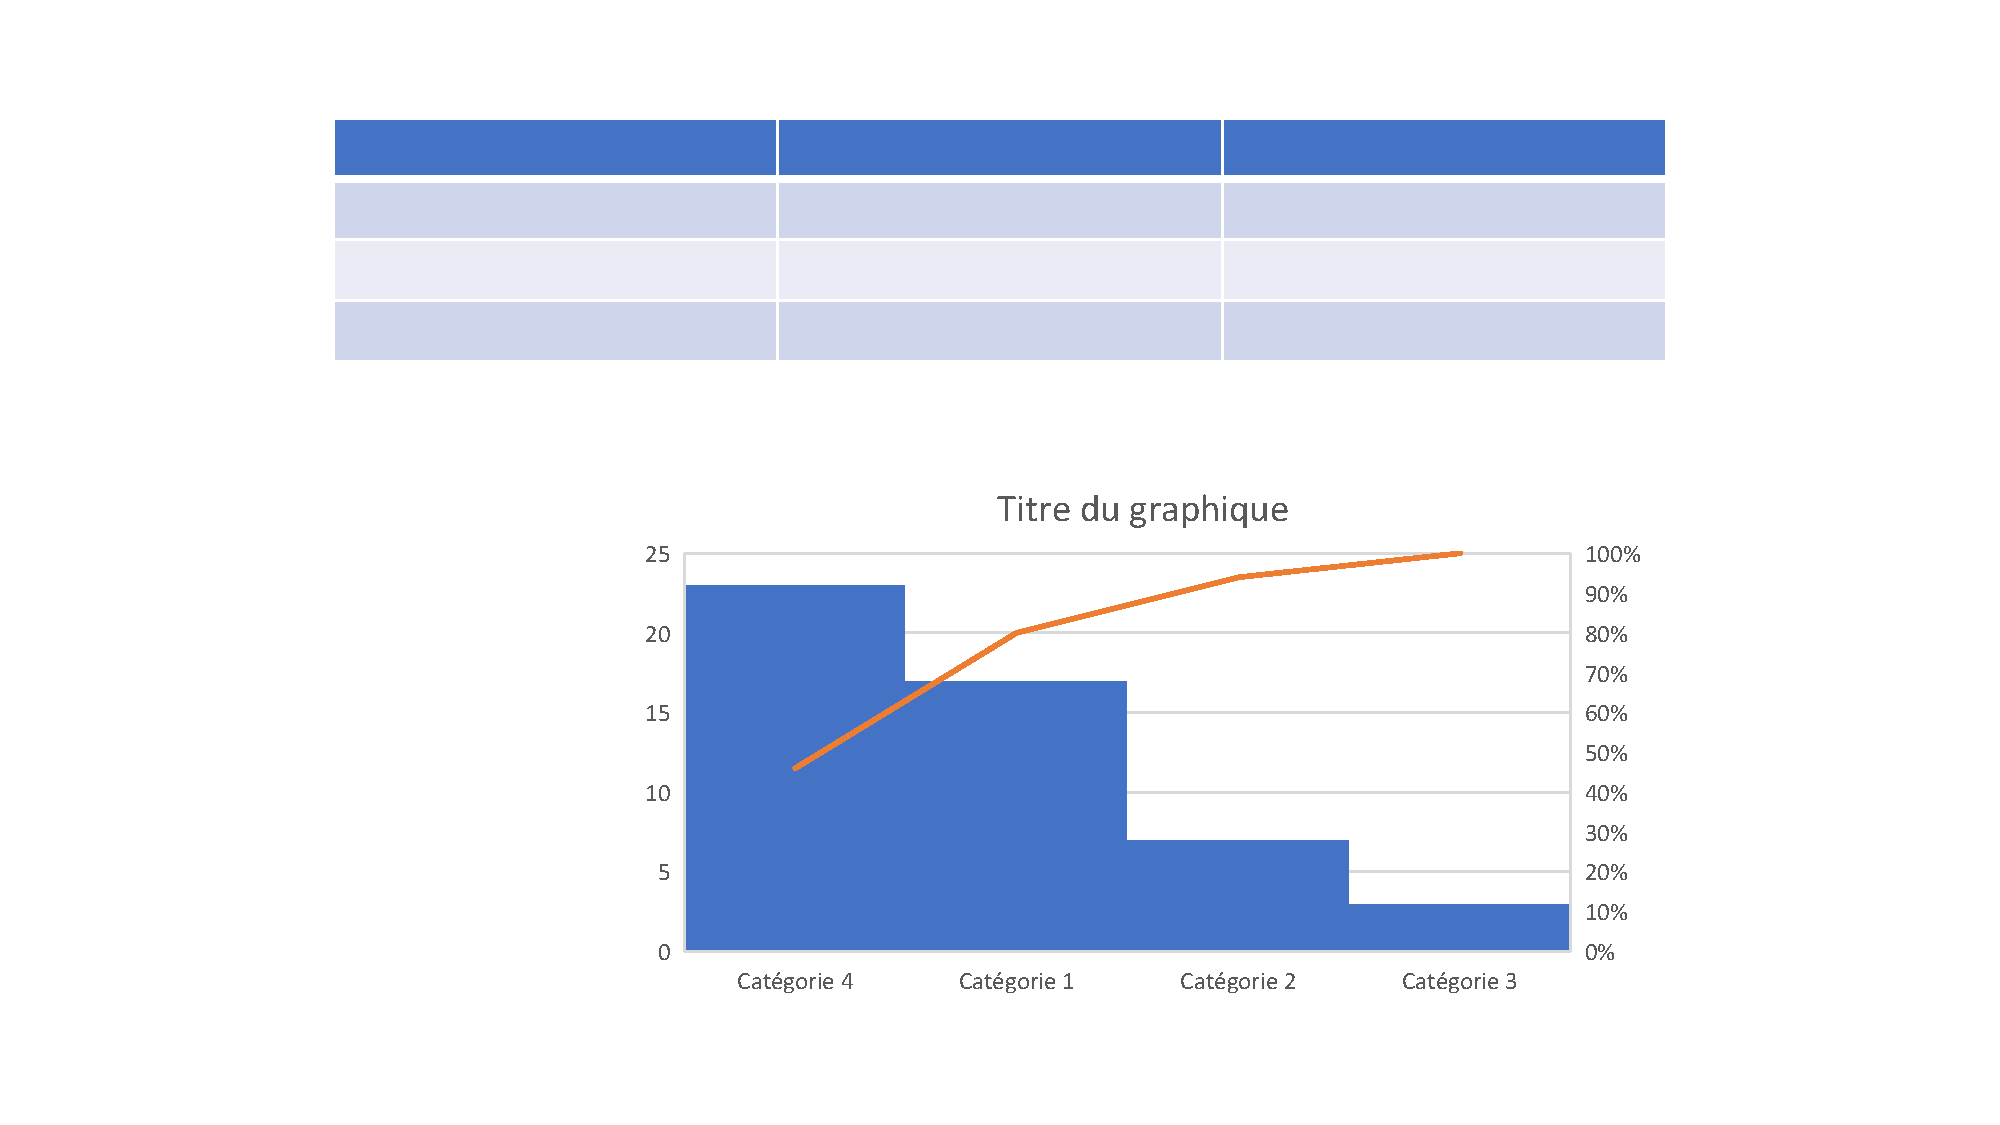
\includegraphics[width=0.50\textwidth]{e_Imagen01}
\caption{Duis eget orci sit amet orci dignissim rutrum.}
\label{fig:particion}
\end{figure}

\section{Tercera sección}
\lipsum[5-6]
                                                          % Resultados
%%%%%%%%%%%%%%%%%%%%%%%%%%%%%%%%%%%%%%%%%%%%%%%%%%%%%%%%%%%%
%% Capítulo 6 / Conclusiones y Perspectivas
%%%%%%%%%%%%%%%%%%%%%%%%%%%%%%%%%%%%%%%%%%%%%%%%%%%%%%%%%%%%
\chapter{Conclusiones y Perspectivas}
\epigrafe{Everyone in this country should learn how to program a computer, because it teaches you how to think.}
              {\textsc{Steve Jobs}}

\section{Conclusiones}
\lipsum[1-3]

\section{Perspectivas}
\lipsum[1]							  % Conclusiones, Perspectivas

%% Apéndices
%%%%%%%%%%%%%%%%%%%%%%%%%%%%%%%%%%%
\appendix	
%%%%%%%%%%%%%%%%%%%%%%%%%%%%%%%%%%%%%%%%%%%%%%%%%%%%%%%%%%%%
%% Apéndice A / Demostraciones
%%%%%%%%%%%%%%%%%%%%%%%%%%%%%%%%%%%%%%%%%%%%%%%%%%%%%%%%%%%%
\chapter{Demostraciones}

\section{Explicando Teorema}
\lipsum[1-2].

\begin{proof} 
  Esta es mi demostración $a \times (b+c)=a \times b + a \times c$ 
\end{proof}
			          % Demostraciones
%%%%%%%%%%%%%%%%%%%%%%%%%%%%%%%%%%%%%%%%%%%%%%%%%%%%%%%%%%%%
%% Apéndice B / Código Fuente
%%%%%%%%%%%%%%%%%%%%%%%%%%%%%%%%%%%%%%%%%%%%%%%%%%%%%%%%%%%%

%%%%%%%%%%%%%%%%%%%%%%%%%%%%%%%%%%%%%%%%%%%%%%%%%%%%% Preparación para el paquete listing
\definecolor{gray97}{gray}{.97}
\definecolor{gray75}{gray}{.75}
\definecolor{gray45}{gray}{.45}

\lstset{ frame=Ltb,
  framerule=0pt,
  aboveskip=0.5cm,
  framextopmargin=3pt,
  framexbottommargin=3pt,
  framexleftmargin=0.4cm,
  framesep=0pt,
  rulesep=.4pt,
  backgroundcolor=\color{gray97},
  rulesepcolor=\color{black},
  %
  stringstyle=\ttfamily,
  showstringspaces = false,
  basicstyle=\small\ttfamily,
  commentstyle=\color{gray45},
  keywordstyle=\bfseries,
  %
  numbers=left,
  numbersep=15pt,
  numberstyle=\tiny,
  numberfirstline = false,
  breaklines=true,
}
% Personalizando los ambientes para listing
\lstnewenvironment{listing}[1][]{
  \lstset{#1}\pagebreak[0]
}
{\pagebreak[0]}
\lstdefinestyle{terminal}{			% Terminal
  basicstyle=\scriptsize\bf\ttfamily,
  backgroundcolor=\color{gray75},
}
\lstdefinestyle{C} {				% Código en C
  language=C,
}

%%%%%%%%%%%%%%%%%%%%%%%%%%%%%%%%%%%%%%%%%%%%%%%%%%%%%%%%%%%%
\chapter{Código Fuente}

\section{Explicando un programa}
\lipsum[1-2]

\noindent
Escribe el siguiente programa en un archivo llamado \texttt{hola.c}:

\begin{lstlisting}[style=C]
#include <stdio.h>

int main(int argc, char* argv[]) 
{
    printf("Hola mundo!");
}
\end{lstlisting}

\noindent
Ahora compila usando \texttt{gcc}:

\begin{listing}[style=terminal, numbers=none]
$ gcc  -o hola hola.c
\end{listing}			          	  % Diagramas

\backmatter

%% Bibliografía
%%%%%%%%%%%%%%%%%%%%%%%%%%%%%%%%%%%
\bibliographystyle{apacite}
\bibliography{biblio}								% Archivo .bib
\nocite{*}

\end{document}